\begin{figure}[htp]
	\centering
	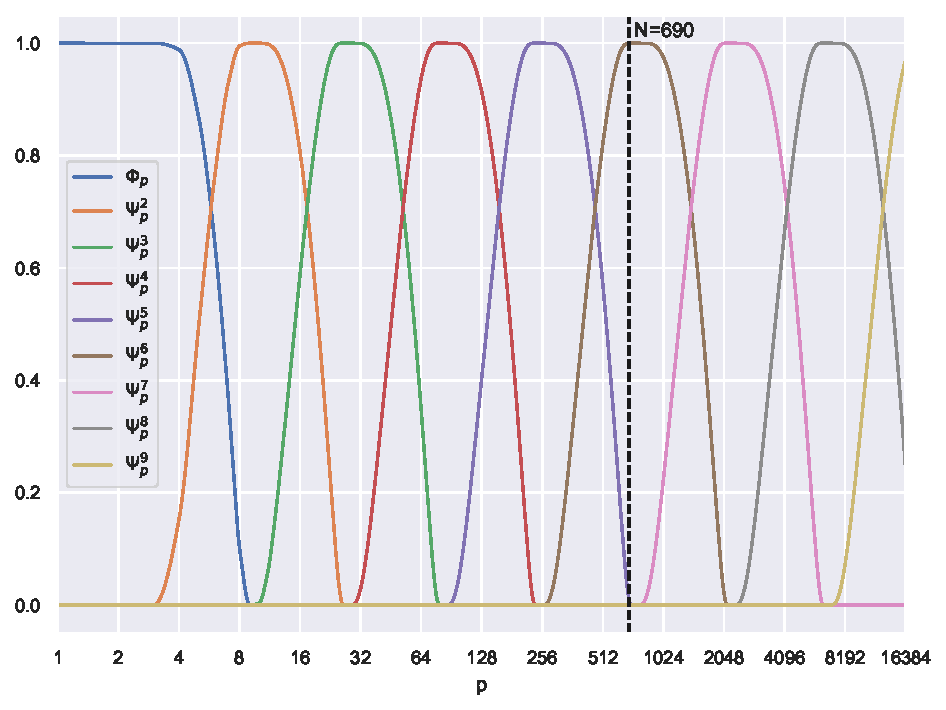
\includegraphics[width=\textwidth]{south_america_slepian_tiling_L128.pdf}
	\caption{
		The tiling of the Slepian line with parameters \(\lambda=3\) and \(J_{0}=2\) with bandlimit \(L=128\).
		The black dashed line marks the Shannon number for the South America region \(N=690\).
		It is clear that the scaling function and the first five wavelets are non-zero as the coefficients are within the Shannon number.
	}\label{fig:chapter3_tiling}
\end{figure}
